%
% teil3.tex -- Beispiel-File für Teil 6
%
% (c) 2020 Prof Dr Andreas Müller, Hochschule Rapperswil
%
% !TEX root = ../../buch.tex
% !TEX encoding = UTF-8
%
\section{Riemannsche Zahlenkugel
\label{moebius:section:teil6}}
\kopfrechts{Riemannsche Zahlenkugel}

Die riemannsche Zahlenkugel dient dazu, die komplexe Ebene um einen zusätzlichen Punkt
\index{riemannsche Zahlenkugel}%
\index{Zahlenkugel!riemannsch}%
\(\infty\) zu erweitern. Diese Erweiterung nennt man die erweiterte komplexe Ebene:
\[
\hat{\mathbb{C}} = \mathbb{C} \cup \{\infty\}.
\]
Dadurch wird es möglich, auch Ausdrücke wie
\[
\frac{1}{0}
\]
sinnvoll zu interpretieren, indem man
\[
\frac{1}{0} = \infty
\]
definiert.
Ebenso gilt
\[
\frac{1}{\infty} = 0.
\]
Allgemeiner betrachtet man Möbius-Transformationen der Form
\[
f(z) = \frac{az + b}{cz + d}.
\]
Der Nenner wird genau dann Null, wenn
\[
cz + d = 0 \quad \Rightarrow \quad z = -\frac{d}{c}, \quad (c \neq 0).
\]
An dieser Stelle wird der Funktionswert in der erweiterten komplexen Ebene als
\[
f\!\left(-\frac{d}{c}\right) = \infty
\]
definiert.
Umgekehrt gilt
\[
f(\infty) = \frac{a}{c}, \quad (c \neq 0).
\]
\\
\subsection{Geometrische Interpretation}
Die erweiterte komplexe Ebene kann geometrisch durch die riemannsche Zahlenkugel dargestellt werden.
Dazu betrachtet man eine Kugel im dreidimensionalen Raum, die die komplexe Ebene im Ursprung berührt.
Der Nordpol dieser Kugel entspricht dem Punkt \(\infty\).
\index{Nordpol}%
Jeder Punkt \(z \in \mathbb{C}\) wird durch die stereographische Projektion auf die Kugel abgebildet:
\index{stereographische Projektion}%
Man verbindet den Punkt \(z\) in der Ebene mit dem Nordpol. Der Schnittpunkt dieser Geraden mit der Kugel ist das Bild von \(z\).
\begin{figure}
	\centering
	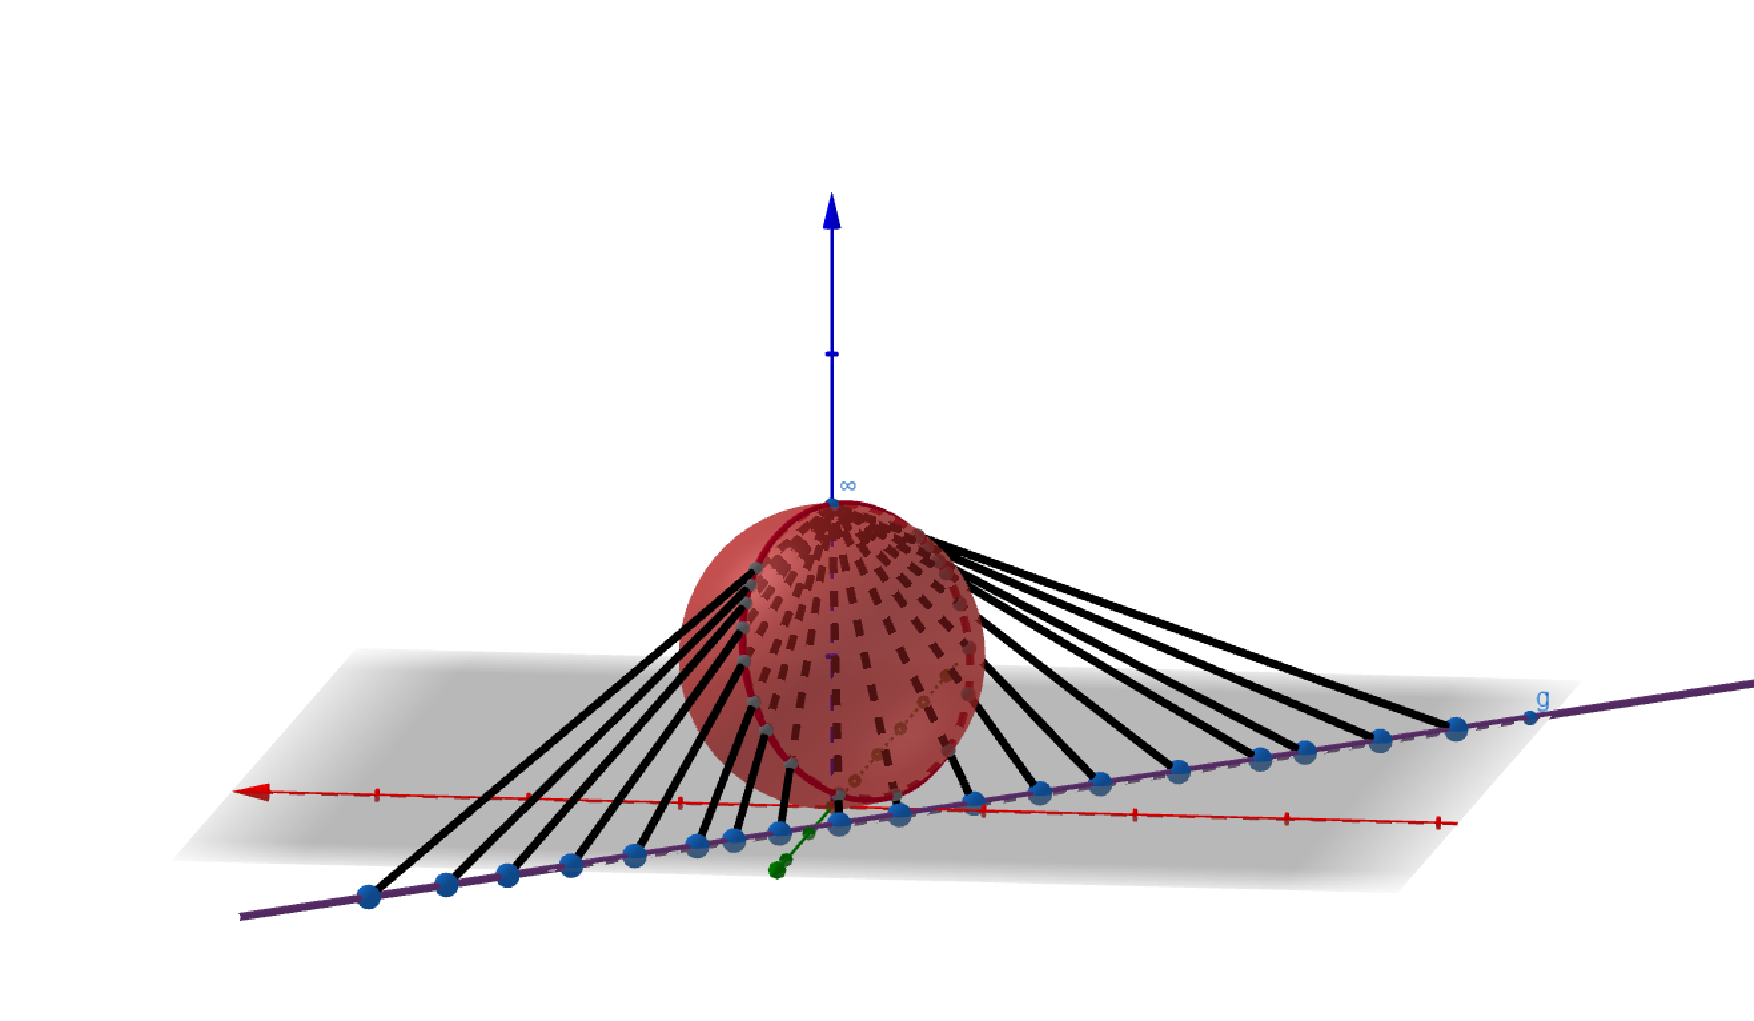
\includegraphics[width=1\textwidth]{papers/moebius/bild8.pdf}
	\caption{Stereographische Projektion einer Geraden (erstellt mit GeoGebra)}
\end{figure}
\medskip

\subsection{Geraden und Kreise}
Ein zentrales Ergebnis ist
\begin{itemize}
	\item Geraden in der Ebene entsprechen Kreisen auf der Kugel, die durch den Nordpol verlaufen.
	\item Kreise in der Ebene entsprechen ebenfalls Kreisen auf der Kugel.
\end{itemize}
Damit gilt:
\[
\text{Geraden und Kreise in } \mathbb{C}
\;\longleftrightarrow\;
\text{Kreise auf der riemannschen Zahlenkugel}.
\]
\begin{figure}
	\centering
	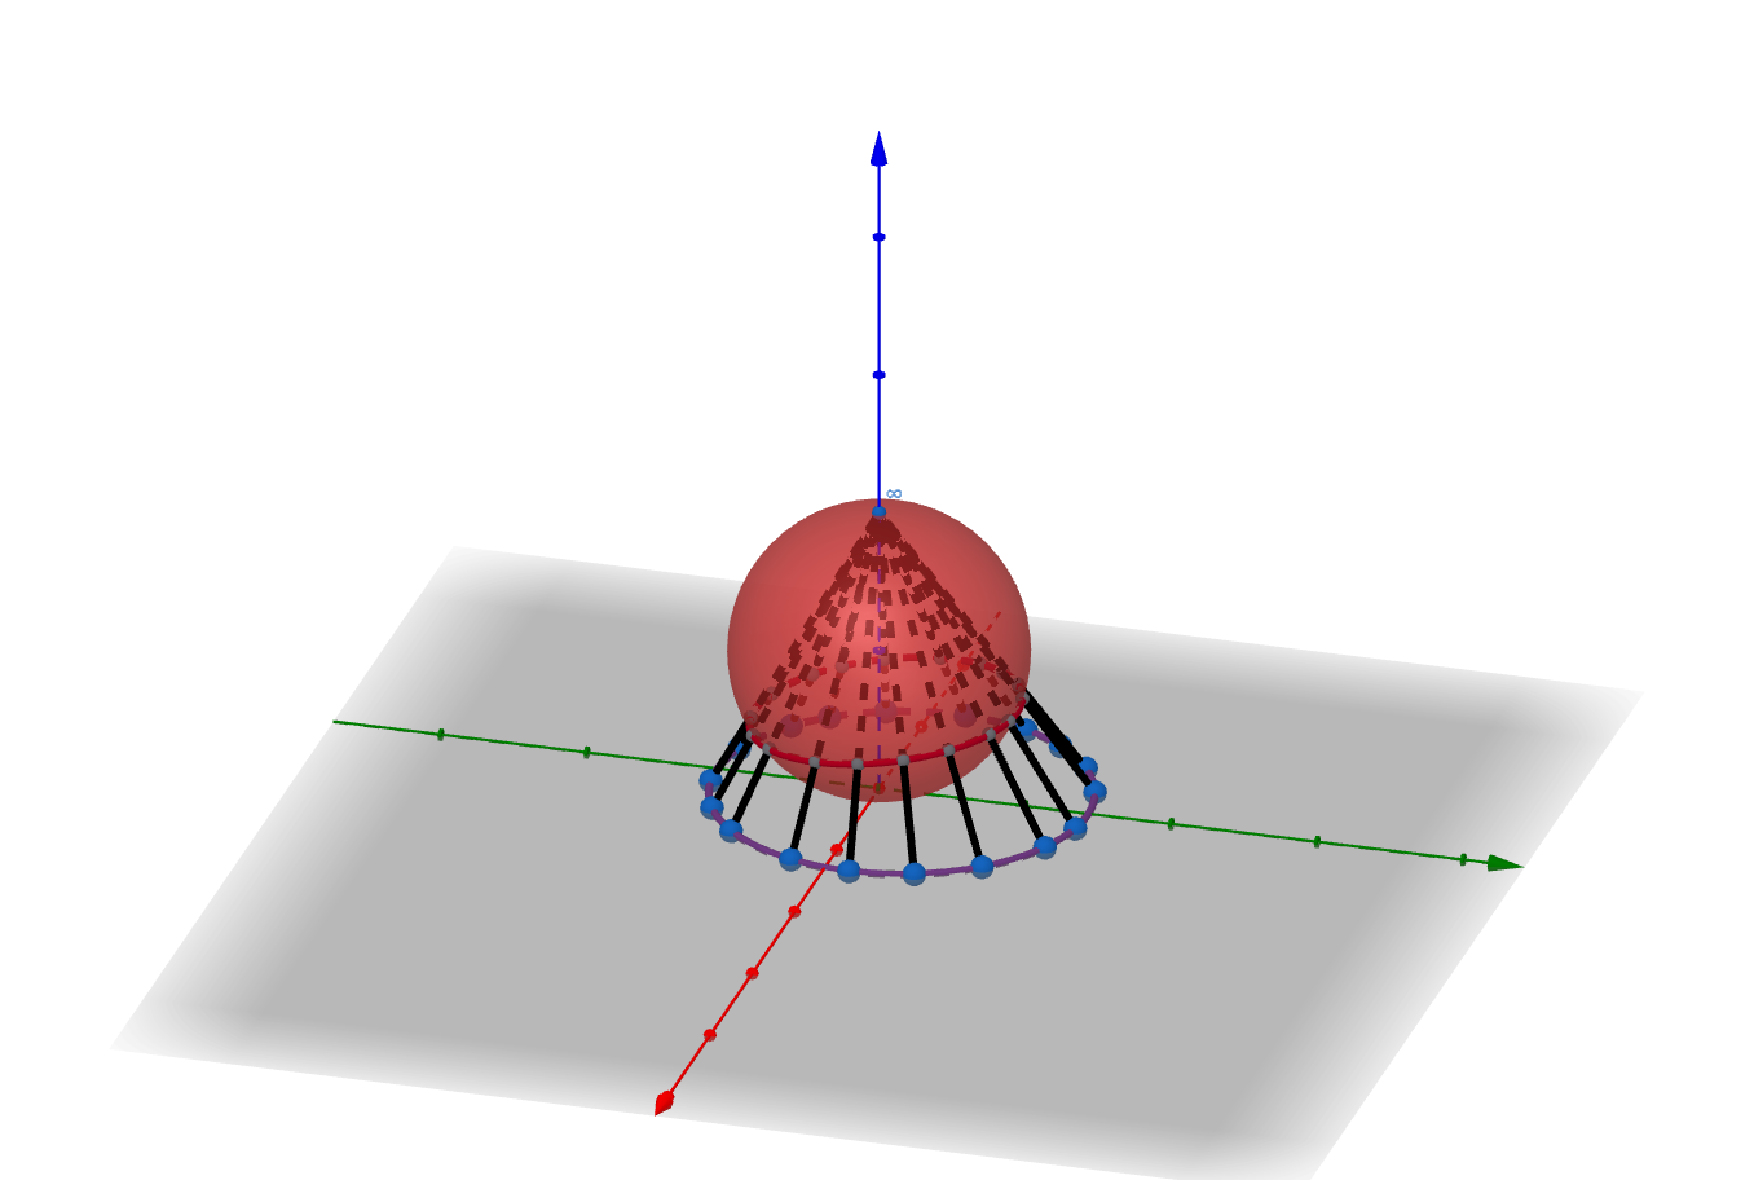
\includegraphics[width=1\textwidth]{papers/moebius/bild9.pdf}
	\caption{Stereographische Projektion eines Kreises (erstellt mit GeoGebra)}
\end{figure}
\\
Zur intuitiven Vorstellung gilt Folgendes:
Man kann sich die riemannsche Zahlenkugel wie eine Weltkugel vorstellen.
In der ebenen Darstellung (wie auf einer Landkarte) erscheinen grosse Kreise oft als Geraden.
Betrachtet man jedoch die Kugel selbst, erkennt man, dass es sich in Wirklichkeit immer um Kreise handelt.
Die scheinbare Unterscheidung zwischen Geraden und Kreisen in der Ebene
ist daher nur eine Folge der Projektion.
 Auf der riemannschen Zahlenkugel werden beide als Kreise vereinheitlicht.
